\chapter{Results}

\section{Depth Camera}

\section{Heightmap}

\section{Walkability Scores}
    For testing the walkability scores described in section \ref{sec:scores}, a piece of terrain that demonstrates various types of obstacles
    that the robot might encounter was chosen, this terrain and its heightmap is shown in figure \ref{fig:score_test_map}.
    \begin{figure}[h]
        \centering
        \begin{subfigure}{.5\textwidth}
            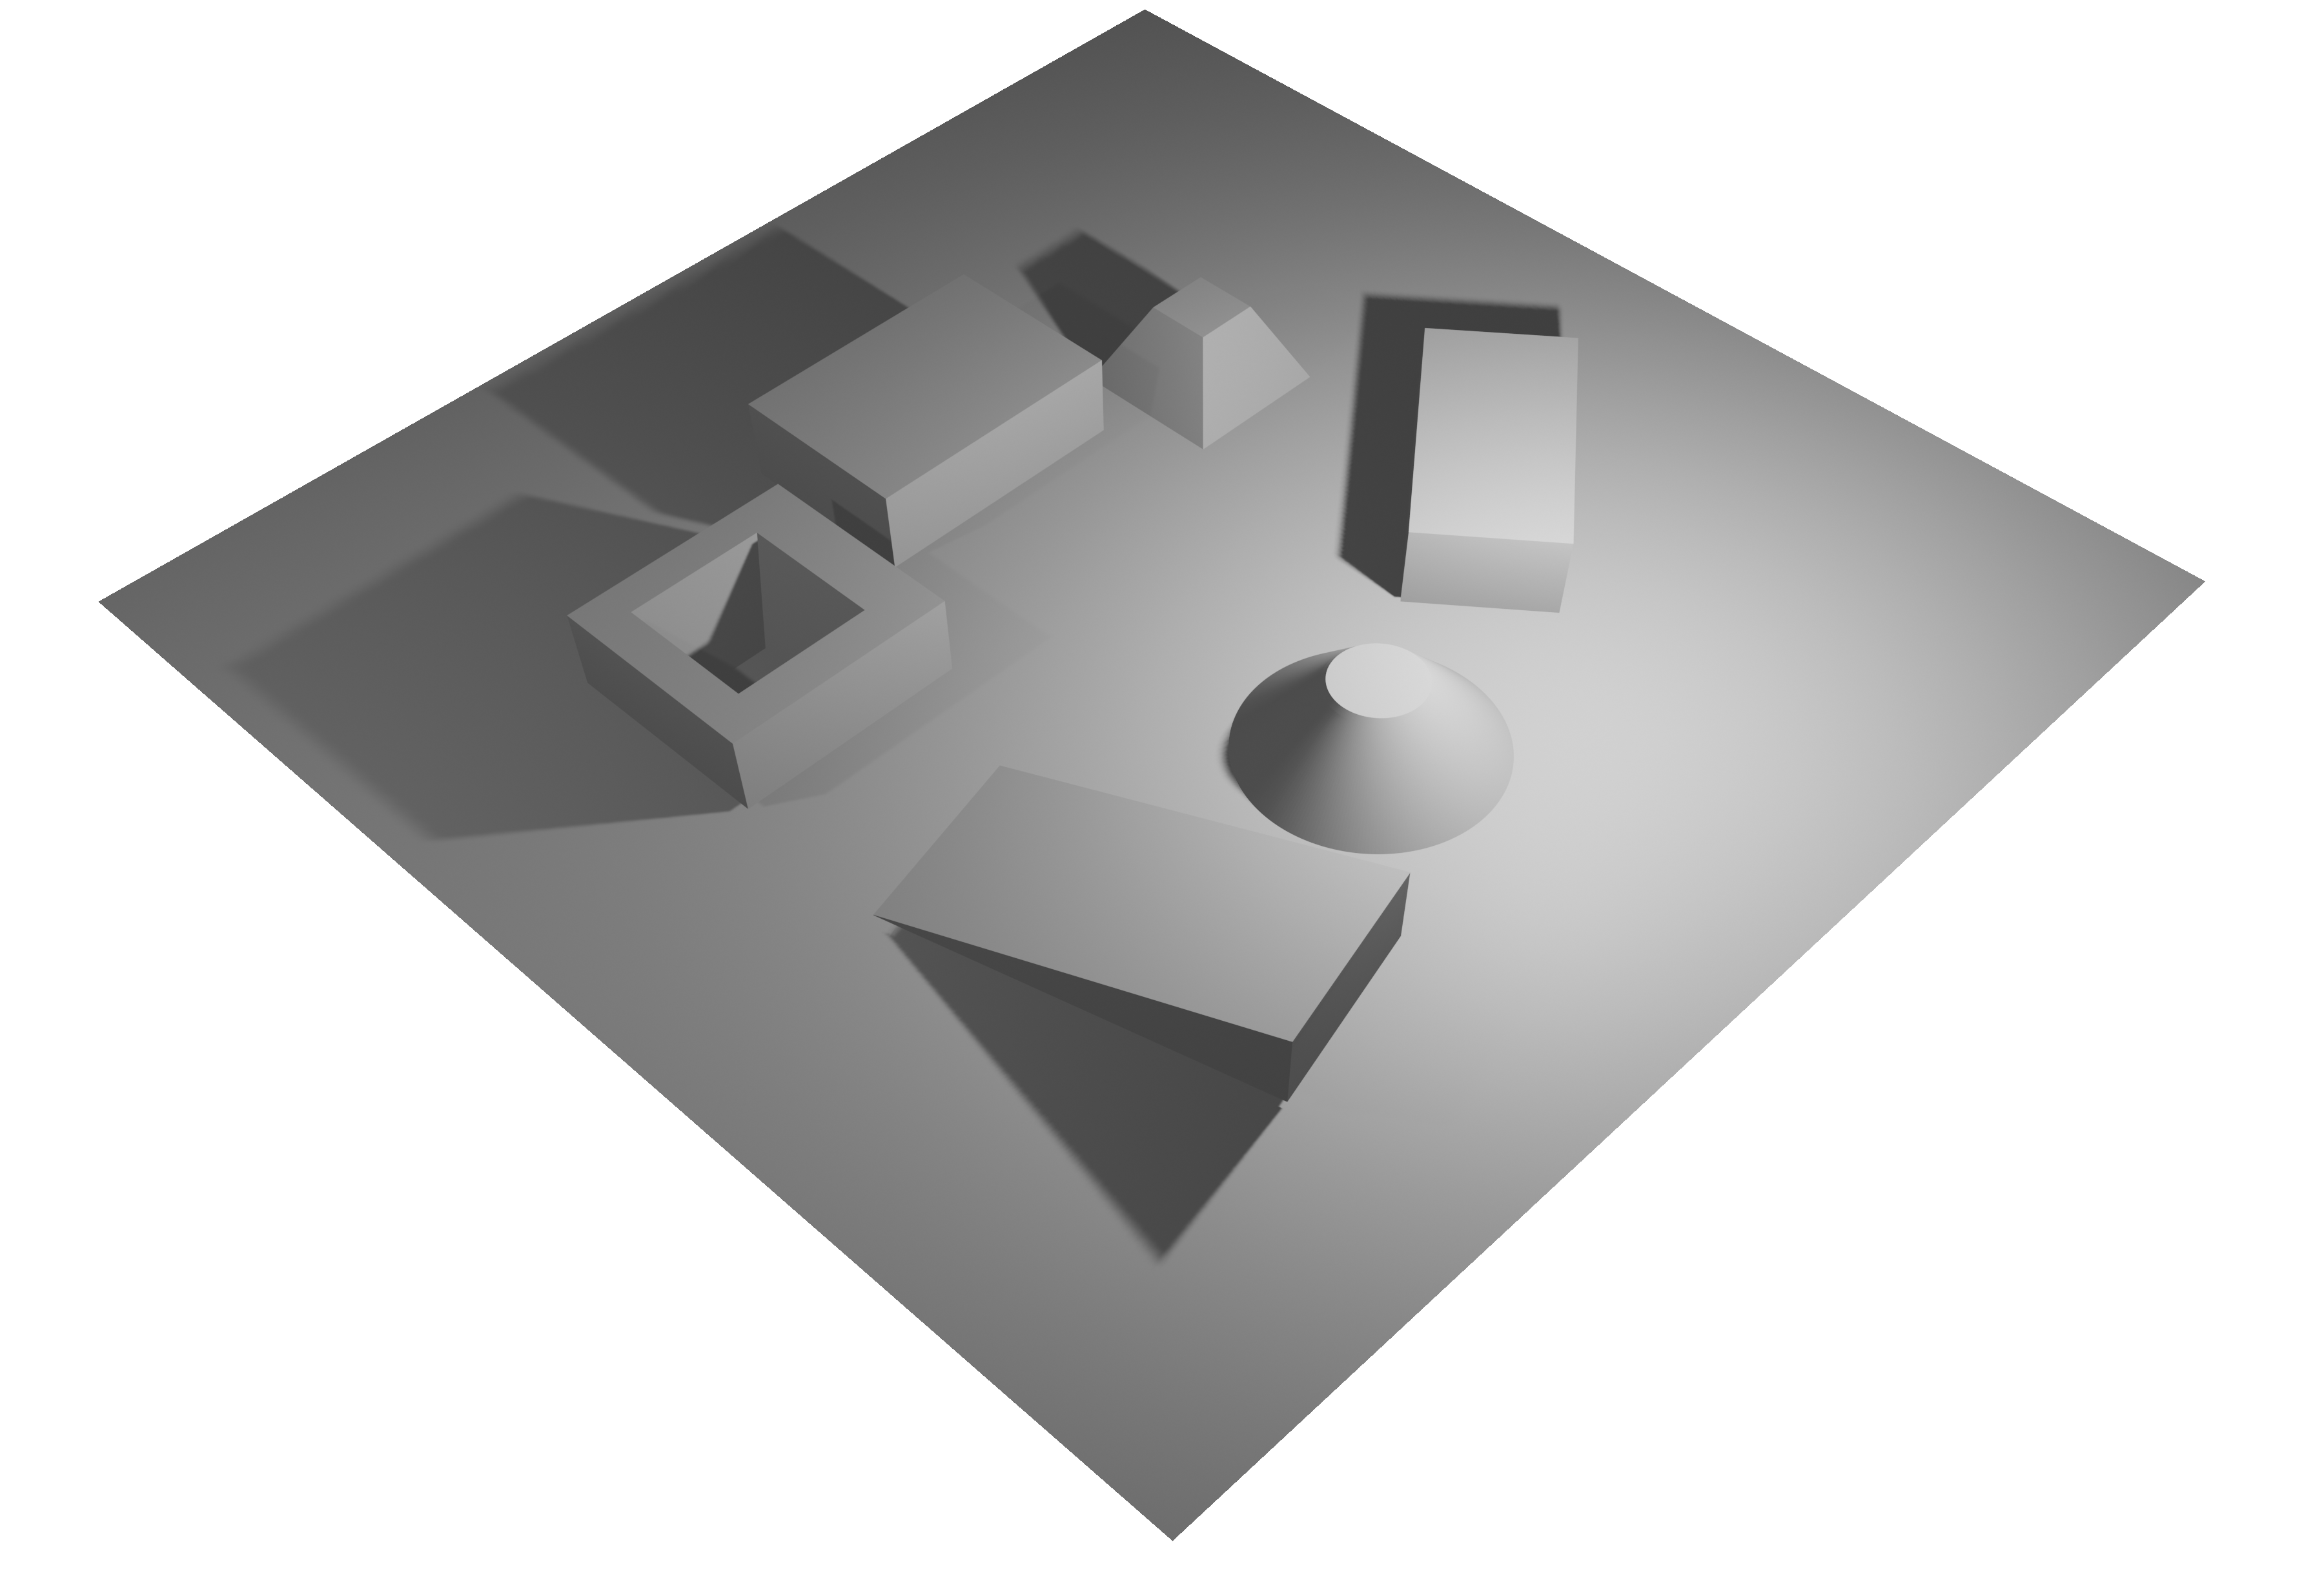
\includegraphics[height=.8\linewidth, left]{hmap3D.png}
            \caption{3D Terrain}
            \label{fig:sub_3d_terrain}
        \end{subfigure}%
        \begin{subfigure}{.5\textwidth}
            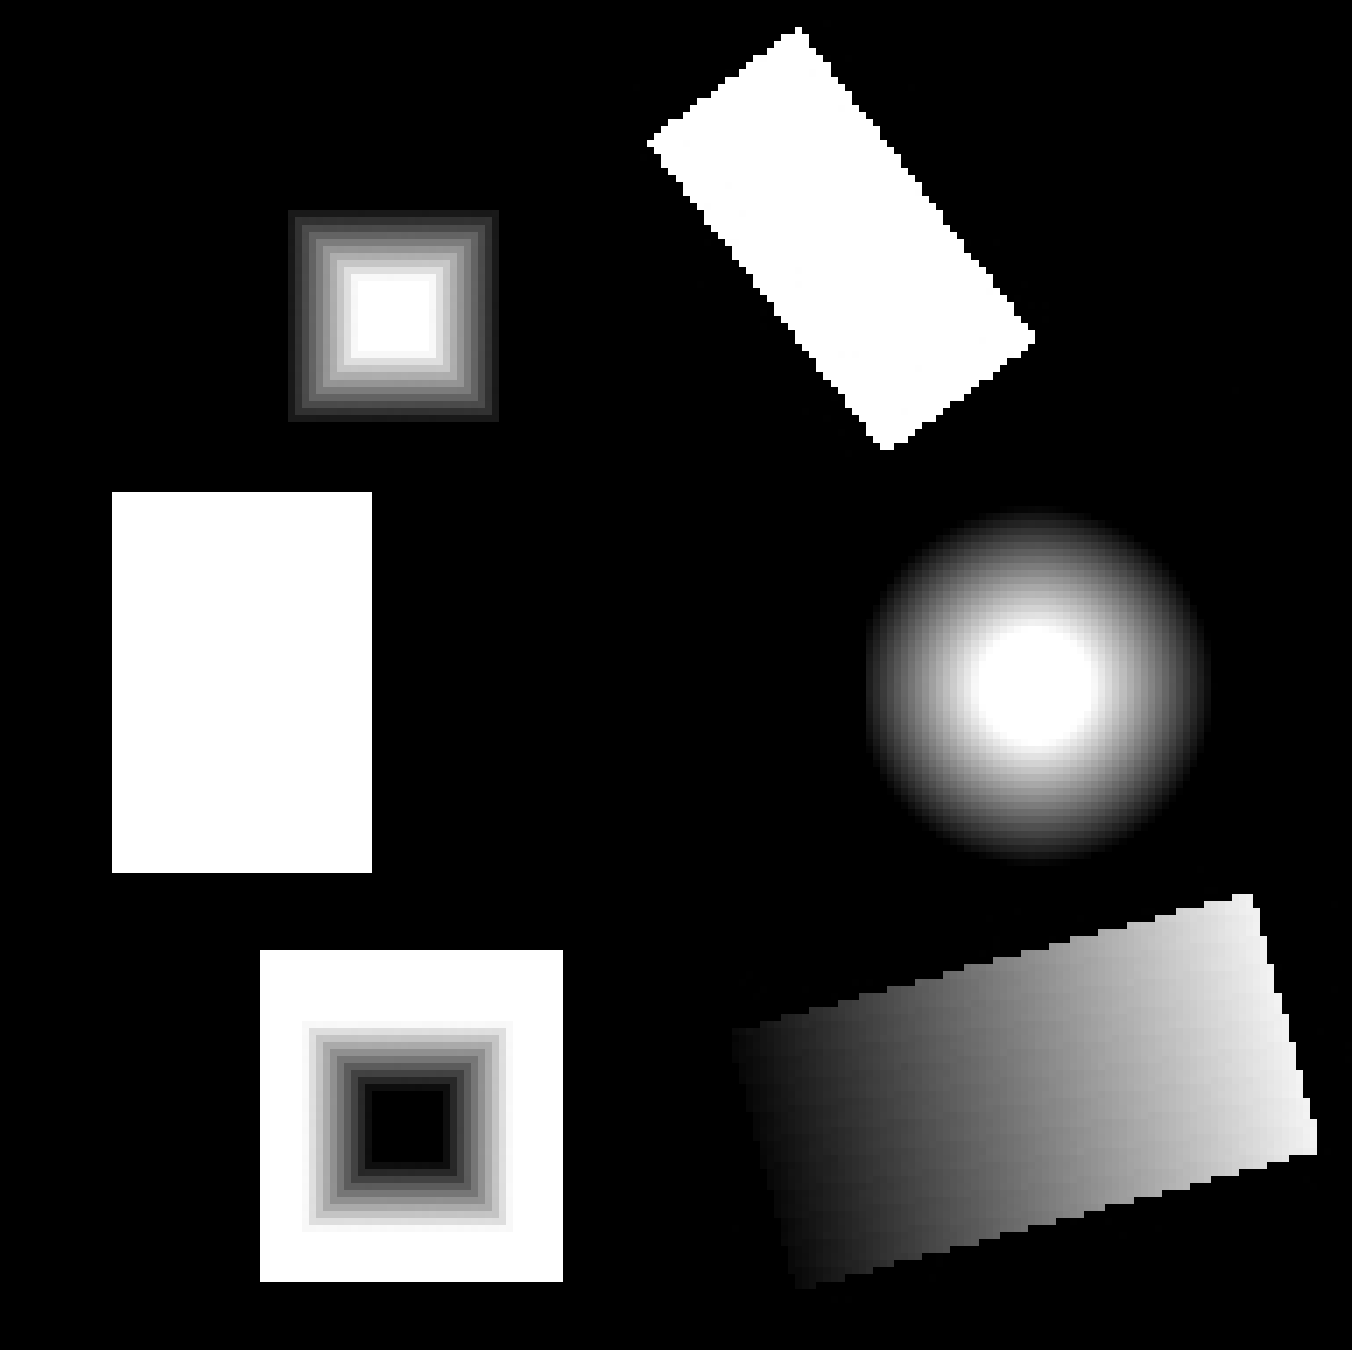
\includegraphics[height=.8\linewidth, right]{scoreTestHmap.png}
            \caption{Heightmap of 3D Terrain}
            \label{fig:sub_3d_terrain_hmap}
        \end{subfigure}
        \caption{3D Model of Terrain and its heightmap.}
        \label{fig:score_test_map}
    \end{figure}
    The heightmap in figure \ref{fig:sub_3d_terrain_hmap} is used to test the various walkability scores, first, in order to show individual results,
    the slope and edge proximity score is applied to the heightmap separately from each other, this is shown in figure \ref{fig:scores_seperate}. Next the combined score is
    shown in figure \ref{fig:full_score}, this is the score that is used to optimise foot end positions.
    \begin{figure}[h]
        \centering
        \begin{subfigure}{.45\textwidth}
            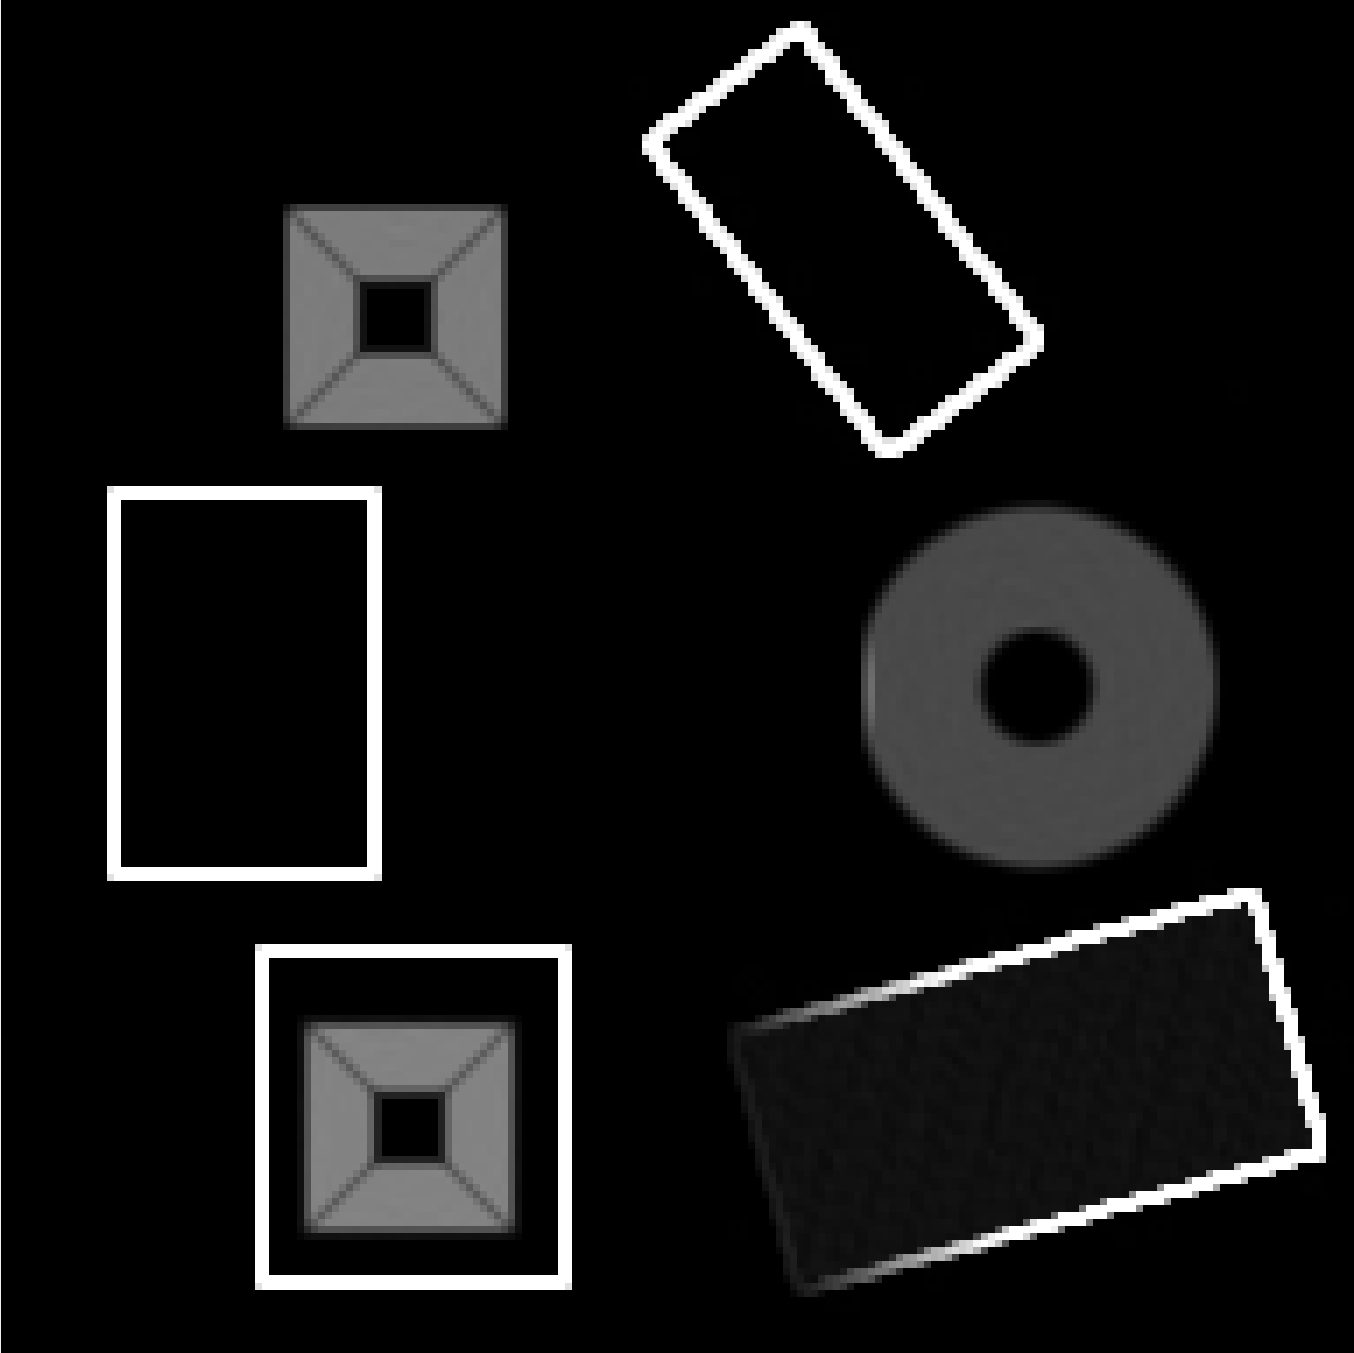
\includegraphics[height=.85\linewidth, left]{slopeScoreTest.png}
            \caption{Slope score test.}
            \label{fig:sub_slope_test}
        \end{subfigure}%
        \begin{subfigure}{.45\textwidth}
            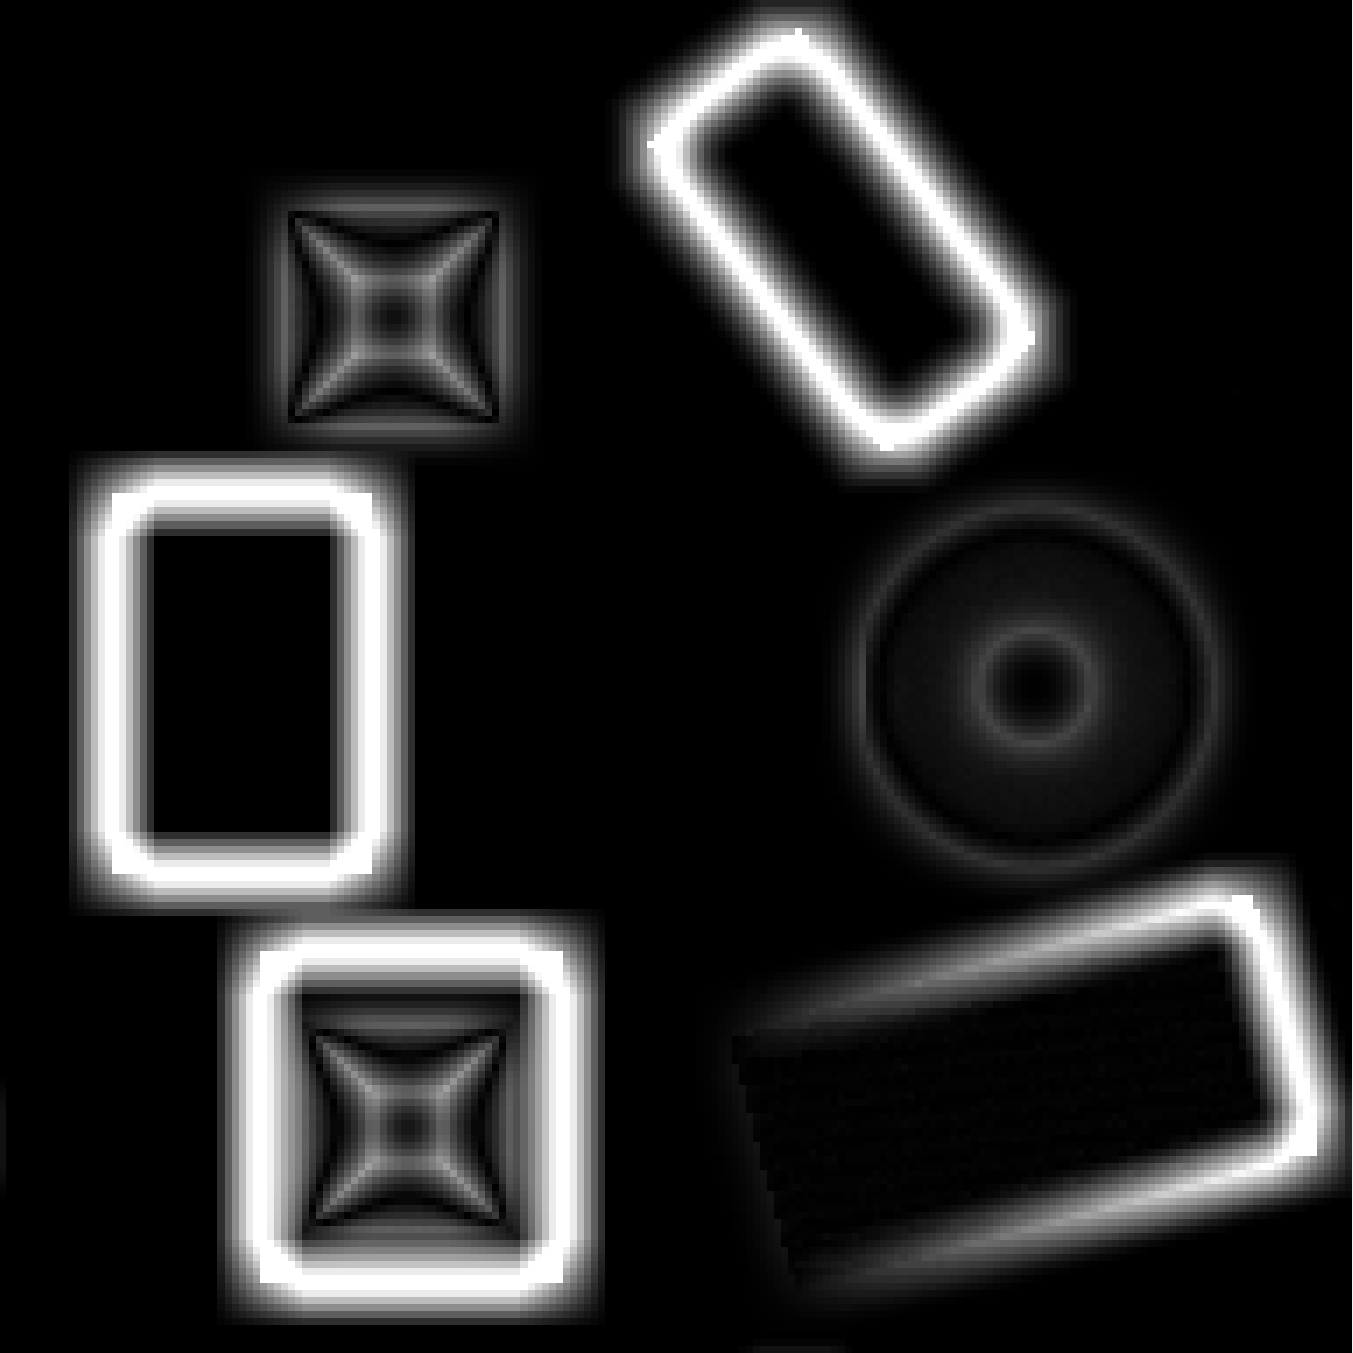
\includegraphics[height=.85\linewidth, right]{proxScoreTest.png}
            \caption{Edge proximity score test.}
            \label{fig:sub_prox_test}
        \end{subfigure}
        \caption{Slope score and edge proximity score tests.}
        \label{fig:scores_seperate}
    \end{figure}
    The slope score can be seen in figure \ref{fig:sub_slope_test}, from this it can be seen that the slope score successfully indicates sloped areas
    as less suitable foot end positions. It is also clear that vertical inclines are strongly discouraged, and while not the primary purpose of the slope
    score, this is expected and does not have a negative impact on scoring.

    Figure \ref{fig:sub_prox_test} shows that edge proximity score successfully discourages foot placement in areas with large height deviations,
    while allowing placement in areas with a locally similar slope, such as the ramp in the bottom-right. As can be seen from the larger, and more intense, discourage areas around the boxes in the
    top-right, bottom-right, left and bottom-left, it is clear that the magnitude of the height differential will increase the size and strength of the rejection area.
    Next, in figure \ref{fig:full_score} the combined slope and edge proximity scores can be seen. This is simply a weighted addition of the two scores.
    \begin{figure}[h]
        \centering
        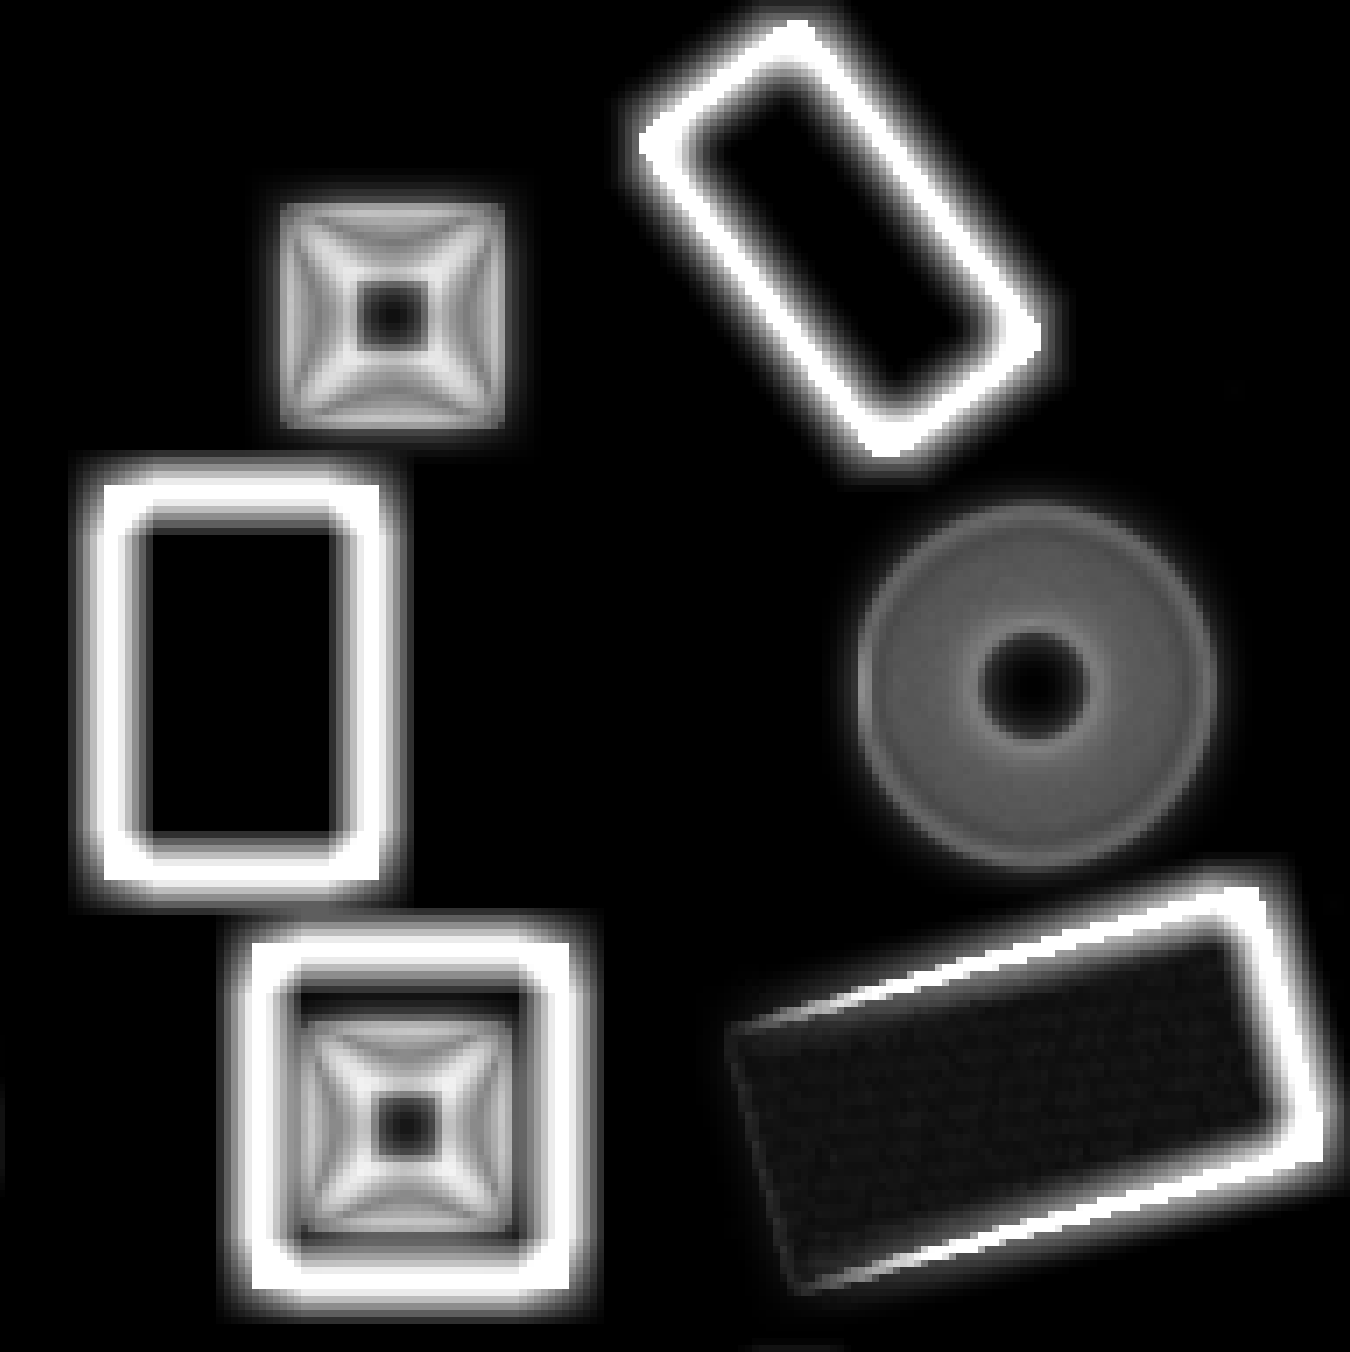
\includegraphics[width=.49\textwidth]{fullScore.png}
        \caption{Full walkability score.}
        \label{fig:full_score}
    \end{figure}

    Finally, the radial search algorithm described in section \ref{sec:radial_search} is used to optimise various nominal foot end positions.
    This is shown in figure \ref{fig:optimisation_test}.
    \begin{figure}[h]
        \centering
        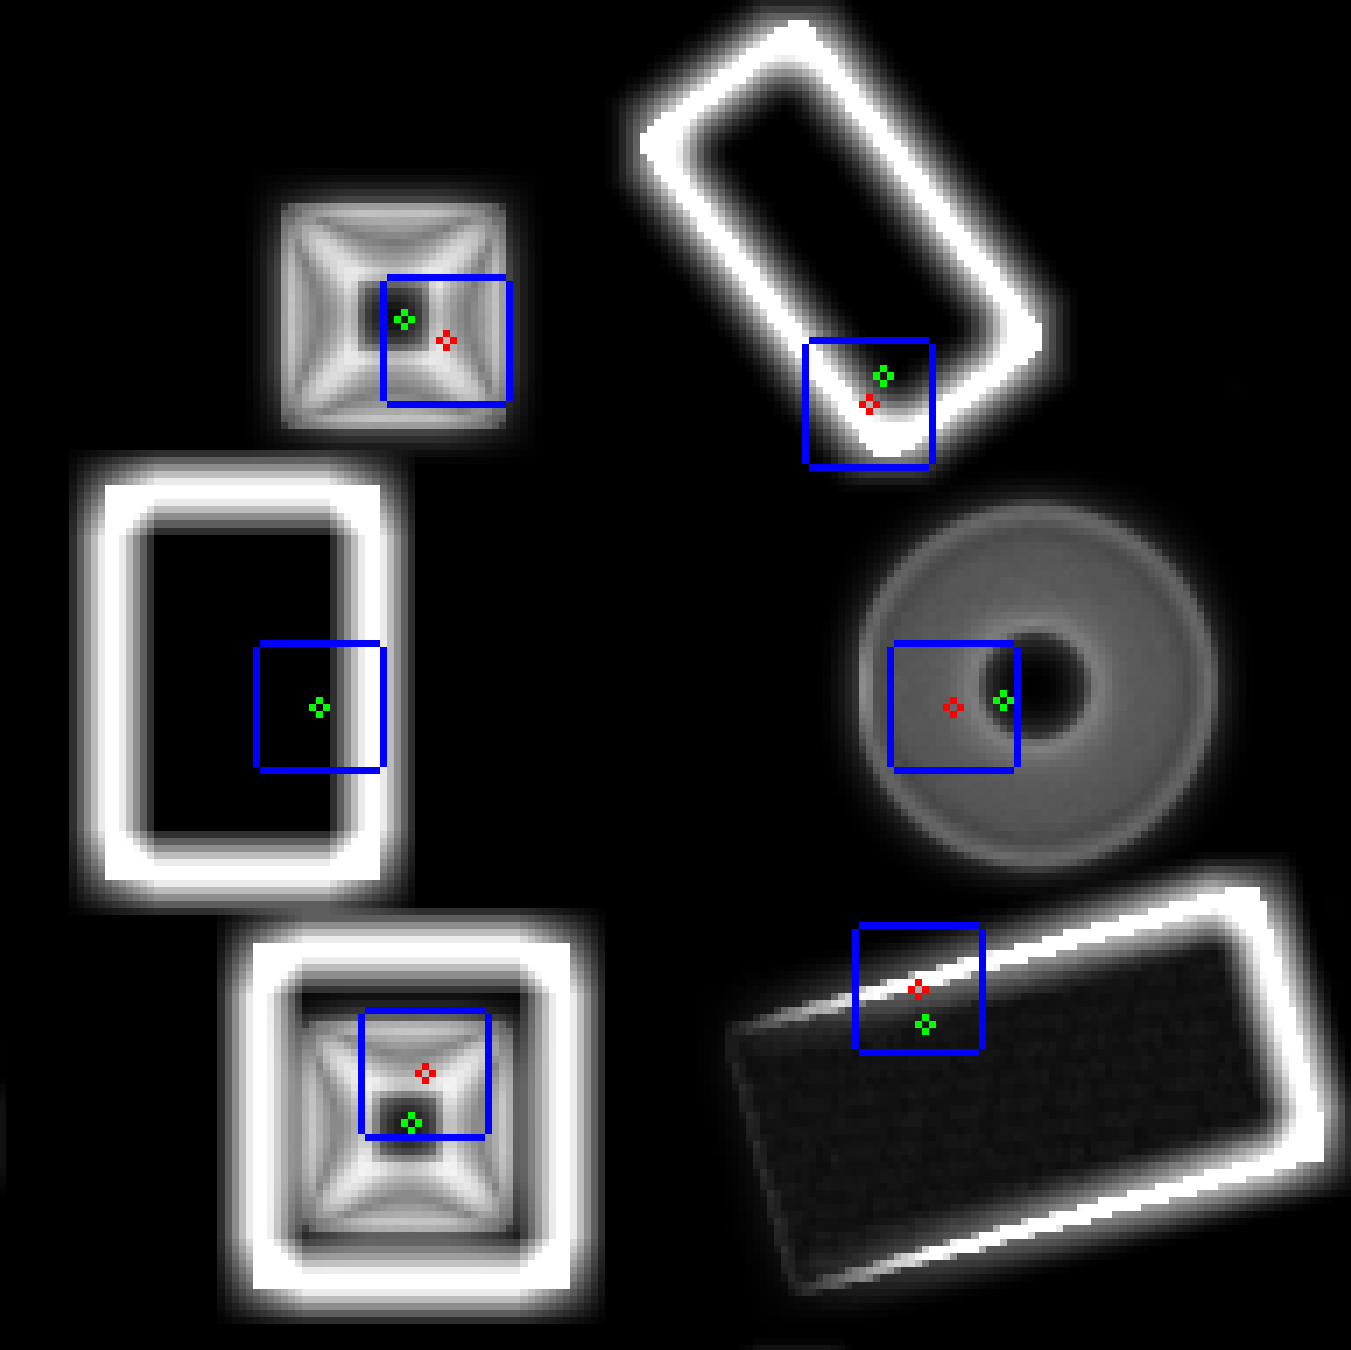
\includegraphics[width=.7\textwidth]{scoreTestFinal.png}
        \caption{Walkability score optimisation test.}
        \label{fig:optimisation_test}
    \end{figure}
    If the nominal foot position is in an acceptable position, the position will not be further optimised, this can be seen with the left most
    nominal position in figure \ref{fig:optimisation_test}. If however the nominal position is too close to an edge, such as with the top-right example, 
    the nominal position is optimised to the closest acceptable position. The optimised position does not need to have a perfect score, as can be seen in the bottom-right example, this example is similar to 
    the aforementioned top-right, but it adjusts onto the ram, which has a non-perfect, however acceptable, walkability score.
    Next the right most example shows how the nominal position is place on a piece of terrain that is too steep, this it is optimised onto the flat surface on top of the round pedestal. 
    
    Finally, the top-left and bottom-left examples show the case of a nominal position placed on a sloped pillar and a sloped hole respectively.
    In both cases the nominal position is optimised to the flat surface at the to of the pillar and at the bottom of the hole.
    
    The flat surfaces on the pillar an in the hole are large enough to not be rejected by the edge proximity score, however, if the inclines sere steeper or the flat surface smaller it is possible that these nominal positions would be
    unsolvable, as there is no appropriate foot end placement inside the search radius. In this case the robot would need to make a course adjustment.

\newpage
\section{Walking}
    The final walking tests are comprised of three different terrains, a simple flat plane as a baseline, then a staircase to demonstrate simple foot and body height adjustment and
    finally a uneven organic like surface.

    \subsection{Flat Plane}
    \subsection{Staircase}
    \subsection{Organic}
    \captionsetup[figure]{oneside,margin={0.9cm,0cm}}
    \begin{figure}[h]
        \centering
        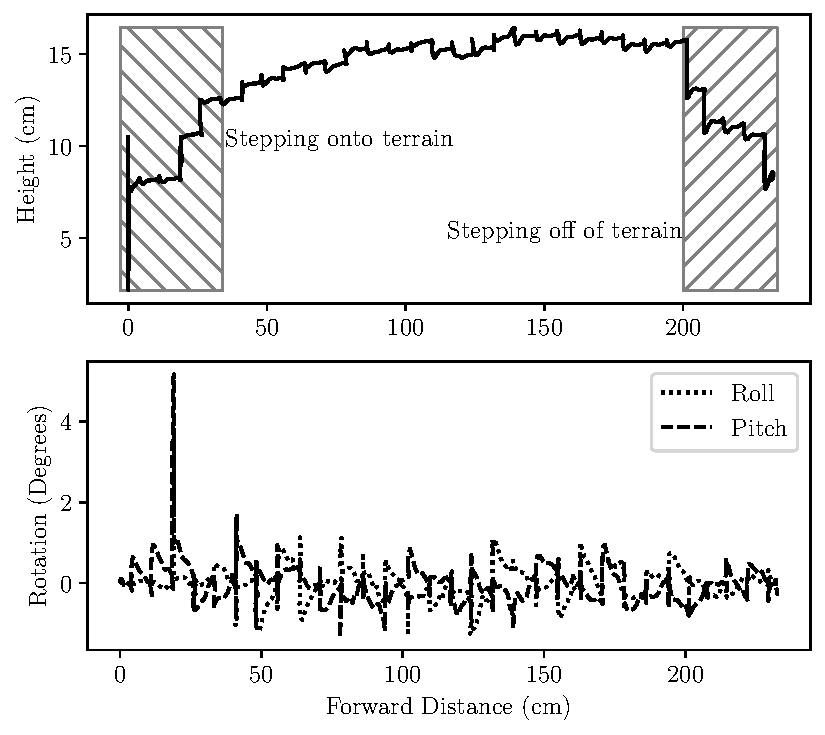
\includegraphics[clip, trim=0 0.25cm 0 0.25cm]{body_data.pdf}
        \caption{Body Data}
        \label{fig:body_data}
    \end{figure}
